\documentclass[12pt,a4paper,english]{article} 
\usepackage{graphicx}
\usepackage{amsmath}
\usepackage{wrapfig}
\usepackage[cm]{fullpage}
\usepackage{layout}
\usepackage{indentfirst}
\usepackage{placeins}
\begin{document}

\title{Flu Forecasting Tool}
\author{Chris Johnson}
\maketitle

Predicting influenza rates has use cases mostly to aid hospitals/urgent care facilities to know how many patients to expect in the up-coming few weeks. In my current position working for Red Oak Sourcing, we are interested in how severe the flu-season from a pharmaceutical stock perspective; making sure there is enough cough/cold/flu related drugs in CVS and CAH supply. That being the case it is most important we accurately forecast the total flu- severity and primary peak location, and we need to do so in the summer time, $\sim 20$-$25$ weeks before the season begins. I present a forecasting model composed of a series of Recurrent Neural Networks (RNNs) that makes 21-week predictions using southern hemisphere influenza data as input.

\section{Introduction}




\begin{figure}[h]
		\begin{center}
		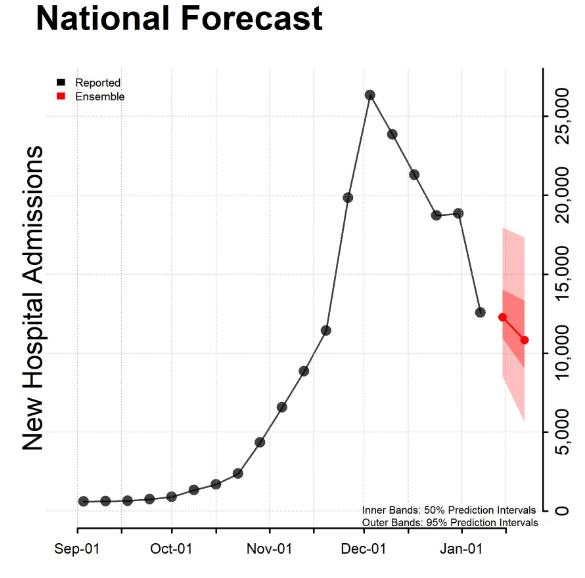
\includegraphics[width=0.45\textwidth]{Pictures/cdc_model.png}
		\caption{CDC model: A one and two-week forecast shown for Jan 7-21 (2023) for combined ensemble models.}
		\end{center}
		\label{fig:cdcc}
	\end{figure}

	
\FloatBarrier



Influenza modeling/forecasting is a famously difficult task due to the constantly evolving virus, vaccine efficacy/compliance among many other factors. If we can reliably forecast the influenza season we can ensure popular cough/cold/flu medications will be gathered and shipped to the parents for patient availability. We have been constructing models to forecast influenza hospitalizations with the belief that more influenza hospitalizations is highly correlated with more flu drug related purchases. To the best of our knowledge, the CDC provides 1-4 week forecasts freely available on their website; our goal is to not necessarily outperform their model, but increase the forecast range. The results presented in this work use $\sim 21$-week lag data so they have up to $21$-week predictive power. This may not give us the total predictive power we desire, but it is 3-4 month improvement of what is available on the CDC website.



\section{CDC}




The CDC pulls together a variety of teams' models and displays 1-4 week forecasts. An example forecast is shown in Figure \ref{fig:cdcc} where Jan-14 and Jan-21 2023 are predicted using data up to Jan-7 2023. I do not attempt to compare my model to the CDC because we are making different forecasts from different data. My goal is to make broader, longer forecasts that can help us decide what ballpark of an impact the flu season will have. I present this CDC model as an example of what is believed to be state of the art, and acknowledge that it does not provide a meaningfully long forecast to be of much use here at ROS. 




\section{Southern Hemisphere Countries}

The countries in the southern hemisphere provide a rough predictive picture of what we can expect in the US due to the phase difference in our seasons.  This model borrows influenza records by every compliant country with the WHO as input into a model that predicts the U.S. hospitalizations records given by the CDC (specifically this is the flu-surv dataset which represents $\sim10\%$ of the population)\footnote{We could just as well have used WHO data as the target as well, but CDC hospitalizations were chosen to avoid bias from having the entire project built on a single data source.}.  

\begin{figure}[h!]
		\begin{center}
		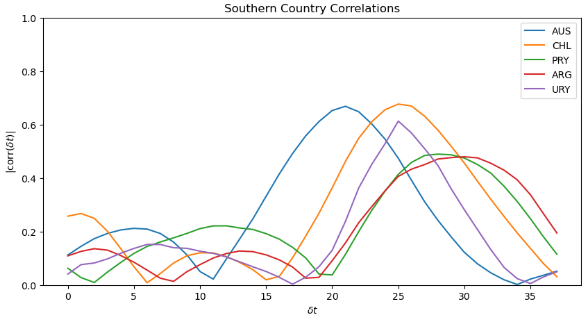
\includegraphics[scale=0.75]{Pictures/so_country_corrs.png}
		\caption{The absolute value of correlations between a select few southern hemisphere country's' influenza case records and the US total influenza hospitalization rates. The correlations are with respect to the number of lagged previous weeks ($\delta t$).}
		\end{center}
		\label{fig:so_corrs}
	\end{figure}
\FloatBarrier

Southern hemisphere countries experience the flu-season approximately half a year out of sync with the US flu-season. Under the assumption the virus moving through the southern hemisphere in the summer is similar to the strand we see come winter, each southern country's flu-season could prove to be a predictive tool for the US flu-season. The WHO provides influenza total counts for a number of countries in the southern hemisphere although some numbers are more complete than others due to poorer countries having inferior health care systems. I display the countries with the highest total correlation with the US hospitalization counts in Figure 2 where $\delta t $ represents the number of week-lags in the southern country with respect to the US. These countries are Australia, Chile, Paraguay, Argentina, and Uruguay. We can see correlation peaks between week lags of $20-30$ weeks out, which would, in principle, allow us at least a 20 week forecast from a given week. I  emphasize that these countries were not chosen to manage the data size to a ``top 5" list, but rather I wish to exclude data that might ``mislead" the model, and cause over fitting, and displaying every country's correlations with the US flu season in one figure is quite noisy.


	

Figure \ref{fig:so_corrs} contains the five southern hemisphere countries most heavily correlated with US flu hospital cases. In this figure, each country case count is normalized to unity for the most severe week.

We can see in figure \ref{fig:so_cases} that although some peaks seam to match in relative strength to the US peak, it is not a complete pattern. For example, the Australia peak for the 2020 and 2022 season seems comparable to the US peak, however in 2018 the peaks are clearly discrepant. We now move to creating models that can make an improved prediction than just examining southern countries by eye.

	\begin{figure}[h!]
		\begin{center}
		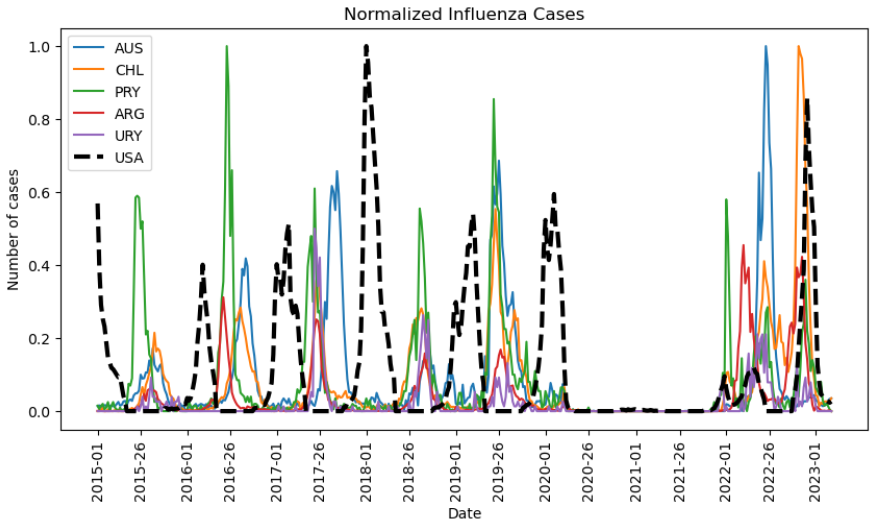
\includegraphics[scale=0.75]{Pictures/flu_cases.png}
		\caption{The US hospitalizations (black, dashed) between 2015 and the beginning of 2023 compared to the 5 southern hemisphere countries total influenza cases documented by WHO. All countries are normalized such that 1 reflects the most severe week that country experienced as documented by the WHO and the CDC.}
		\end{center}
		\label{fig:so_cases}
	\end{figure}
\FloatBarrier
\section{Models}
In this section I motivate and describe the models that I believe to be promising, other models that performed poorly are left out, and we emphasize we have merely scratched the surface of model choices. This section can be a little dense with the detail, so if the reader wishes to just skip to the results they can move onto the next section.
\subsection{Linear-Random Forest}

The first model is a residual hybrid architecture featuring the linear regression and the extreme gradient boosted trees. We combine these models by training a linear model with one set of features, and training a random forest with another set of features on the residual with the target and the linear model. Combining these two models in a time-series forecast is fairly standard practice with the belief that including the two together finds a balance between the under (over) fitting properties of linear (random forest) models to properly capture trends.

I separate the features included into two categories; parameterized seasonal features, and country features. The parameterized seasonal features only depend on the week $t$, and the country features depend on specific data given by other countries at previous weeks. The parameterized seasonal features have Fourier components of the type $\sin(t n\pi/52),\cos(t n\pi/52)$ to capture the yearly seasonal behavior of the flu. To be clear, this is a linear model in model parameters $\vec{\theta}$, not necessarily time $t$. The linear model looks like the following,

\begin{equation}
y = \theta_0 + \sum_n\left( \theta^{sin}_n\sin(\phi + n\pi t/52)+\theta^{cos}_n\cos(\phi+n\pi t/52)\right)
\end{equation}

which is clearly linear in $\vec{\theta}$. The sum over $n$ is not all inclusive, we have selectively removed poor periodic modes. Seasonality with a week date-time index does bare the problem that a year is not exactly 52 weeks, we explore other options in the next section. We applied a mask to the Fourier terms to zero them during the first COVID year accounting for the anomaly in the seasonal pattern.

The country features are the normalized lagged country influenza counts described in the previous section. Each country lags were chosen based off the width of their correlation curves in Figure \ref{fig:so_corrs}, and are displayed in table \ref{tab:lags}.

\begin{table}[h!]
\begin{tabular}{cc}
Country & Lags \\
\hline
Australia & $25\pm 5$ \\
Chile & $25\pm 5$ \\
Paraguay & $27\pm 5$\\
Argentina &$ 30\pm5$ \\
Uraguay &$ 24\pm 3$
\end{tabular}
\label{tab:lags}
\caption{Country week lag centers with their range in both directions.}
\end{table}

In addition to the country lags, an exponentially smoothed version with a smoothing of $\alpha = 0.075$ was included as well. Exponential smoothing is a weighted moving average, with $\alpha= 0 $ including all previous terms evenly, and $\alpha=1$ is no averaging at all. This number was experimentally tuned, but more optimization is certainly an avenue to pursue. For completeness, the linear portion of the model now looks like the following,

\begin{align*}
y_{lin} &= \theta_0 + \sum_n\left( \theta^{sin}_n\sin(n\pi t/52)+\theta^{cos}_n\cos(n\pi t/52)\right)+\sum_{country}\left(\sum_{t_{country}}\theta^{country}_{t_country}y_{country}(t_{country})        \right) \\
&+ \sum_{country}\left(  \sum_{t_{country}}\theta^{country_{exp}}_{t_{country}}y^{exp}_{country}(t_{country})  \right)     
\end{align*}

where $t_{country}$ represents all of the week lags included for each country.

A first round of fitting is done for the linear model described by the equation above, subsequently the residual is now de-seasonalized (model captures the basic periodic behavior). This residual $y_{resid} = y_{lin} - y$  is then used to fit the decision tree model, but only using the country features to, anecdotally speaking, find the combinations of the data that the linear model may have missed. The seasonal features are adequately described with the linear model and are not needed to be included in the second stage of fitting.



\subsection{RNN}


We employ RNNs to utilize feedback connections that enable them to learn long sequences of data where ordering is important. These have the particular advantage of not needing a parametric description to capture the seasonality. The input features the 5 southern countries and the US influenza cases in batches of 26 week long sequences shifted by 20 weeks. 

%\begin{wrapfigure}{r}{0.5\textwidth}
%		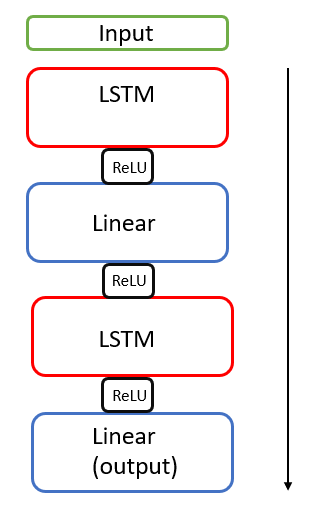
\includegraphics[width=0.25\textwidth]{Pictures/lstm_diagram.png}
%		\caption{A visual representation of the neural network. Features an input followed by LSTM (sequence length = 26), a linear layer (26x26), another LSTM (sequence length = 26), an output layer (output dim = 1), with ReLU activation between each layer.}
%		\label{fig:lstm_diag}
%	\end{wrapfigure}
	
The architecture of the models follows the general recipe
\begin{equation}
o^t = \mathbf{i}^t_{\mu\nu}\mathbf{A}^{t}_{\mu\nu,\mu'\nu'}\mathbf{B}^{t}_{\mu'\nu'}
\end{equation}
where the separable pieces $\mathbf{A}^t,\mathbf{B}^t$ are defined as 
\begin{align}
\mathbf{A}^t_{\mu\nu} &=\left(\prod_{n} \mathbf{RNN}^{t,n}_{\mu'\nu'}\mathbf{ReLU}^{t,n}_{\mu''\nu'',\mu\nu''}\mathbf{Lin}^{t,n}_{\nu''\nu}\right)\\
\mathbf{B}^t_{\mu\nu} &=\mathbf{Flat}^t_{\mu'\cdot\nu' \equiv \sigma} \left(\prod_n\mathbf{ReLU}^{t,n}_{\sigma,\sigma'}\mathbf{Drop(0.05)}\mathbf{Lin}_{\sigma',\nu}\right)
\end{align}
This is an input tensor of shape $[T_{window},26,6]$ where $T_{window}$ is the total weeks included in the fitting procedure. In other words for a given week $t$, there will be $t-20,t-21,...,t-(20+26)$ sequenced data. This shift allows us to predict a data point that is 20 weeks away from the time the data is collected, and the sequence of 26 weeks is chosen such that is a sufficiently long enough window for the RNN to learn the pattern. The network is pictorially represented in figure \ref{fig:lstm_diag} which features a RNN network follow of 26 week sequence length, followed by a linear layer (26x26), another RNN unit of 26 week sequence length, and finally an output linear layer with rectified linear units applied between each layer.


	
\section{Results}
We now discuss the models qualitatively in how well they predict the highest peak severity, location (week of the most cases), and width (when does the season start and end).
\subsection{Hybrid model}

	\begin{figure}[h!]
		\begin{center}
		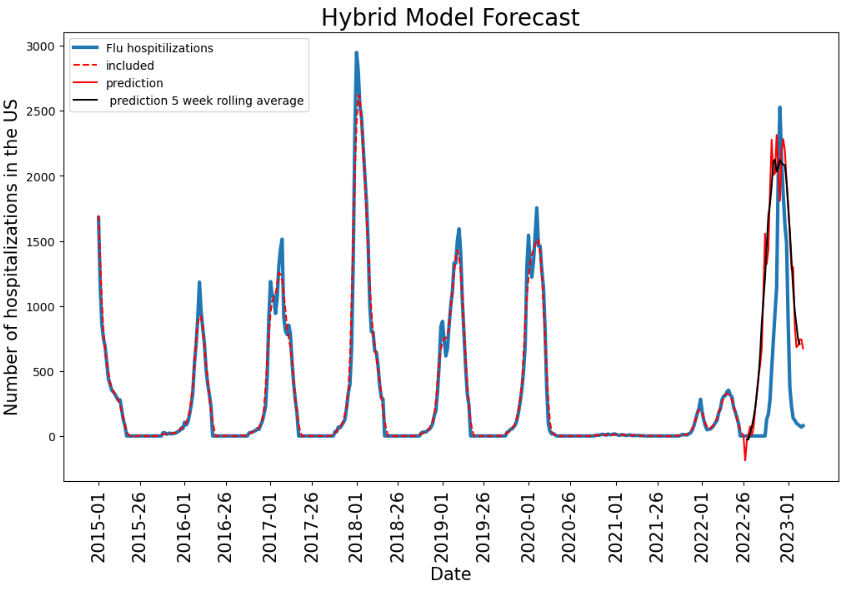
\includegraphics[scale=0.5]{Pictures/hy_model.png}
		\caption{Hybrid model results (red), the data used in the training is dashed. The black line is a 5-week centered rolling average of the result.}
		\end{center}
		\label{fig:hy_model}
	\end{figure}
\FloatBarrier

To train the model we used data ranging from the first week of 2012 to week 26 of 2022, spanning a little more than 10 years. Week 27 of 2022 through 23 were not included in the model and serve to display how well the model can actually forecast. The results are displayed in Figure 5 in a raw (red) and rolling averaged form (black). 

We can see that the peak severity is mostly captured by the model, as well as the center, but not the width of the season. So we would conclude as it stands this model checks 2 of the 3 boxes. 


%\subsection{LSTM}


	\begin{figure}[h!]
		\begin{center}
		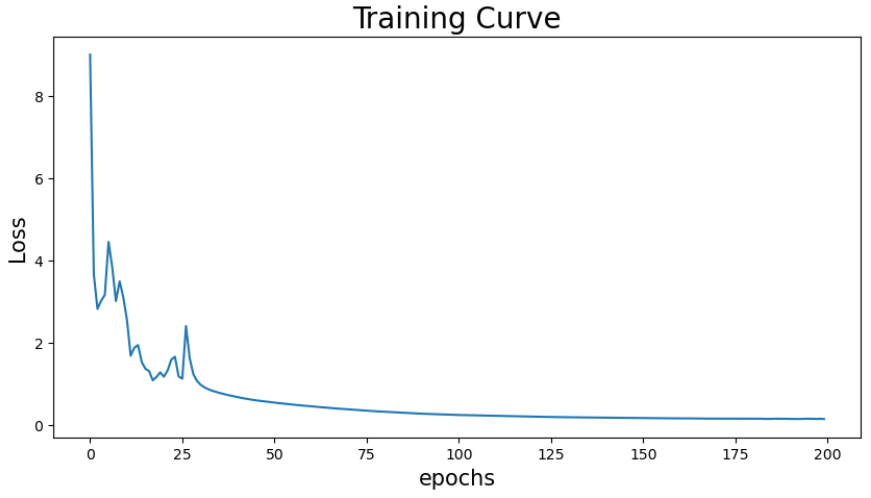
\includegraphics[scale=0.6]{Pictures/flu_train.png}
		\caption{Training curve for LSTM model. This is a mean-squared-error loss function.}
		\end{center}
		\label{fig:lstm_train}
	\end{figure}
\FloatBarrier


	\begin{figure}[h!]
		\begin{center}
		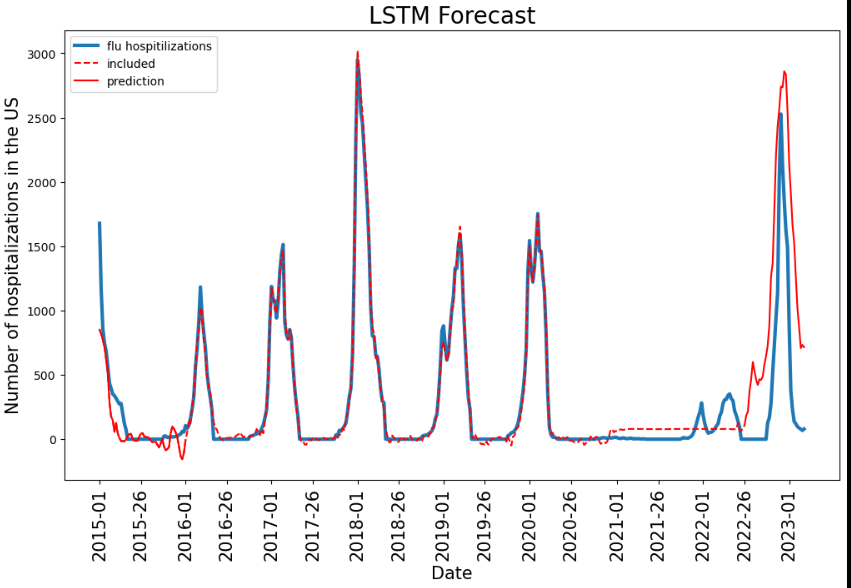
\includegraphics[scale=0.6]{Pictures/lstm_model.png}
		\caption{LSTM model results (red), the data used in the training is dashed. Notice 2015-2016 was also not included in the training set.}
		\end{center}
		\label{fig:lstm_model}
	\end{figure}
\FloatBarrier

Training neural networks requires minimizing a ``loss" function (a formula that reflects how in agreement a model is with the data). Figure 6 demonstrates that as the model ``learns" the data the loss function decreases and eventually plateaus. This minimum point reflects that the model can no longer improve or only modestly improve the description of the data. We can see the result of the model in Figure 7 where I have used 2016-01 (week 1 of 2016) through 2022-26 (week 26 of 2022) as input data to train the model. After 2022-26 is the models 20 week forecast. By this I mean each data point was predicted from 20 week old data so that in principle, one can forecast a flu peak before it occurs. We can see that the model does describe the peak near 2023-01 quite well, the severity, peak location and width all pass the eye-test. The model does lack the ability to capture the little bumps before hand, but I claim that is actually reassuring. If we revisit figure \ref{fig:so_cases} we see that there was no flu activity in any of the southern countries between 2020-01 and 2021-50. So the model did not ``invent" something that was not there. Likely there was no flu activity in this time period for pandemic related reasons, whether it was extensive lock-downs or just under-reporting.

\section{Conclusion}

Figure 8 displays the two ``promising" models together, and sum of the current status of the project. There is much more model experimentation that needs to be performed, if I can produce a variety of models that predict well than I can make forecasts that are more resistant to model bias. I emphasize that flu modeling is difficult, and this is merely meant to be another tool in the toolbox. As for implementing the tool, I envision this as potentially another dashboard that displays the current model results, updating each week when new flu data arrives.


	\begin{figure}[h!]
		\centering
		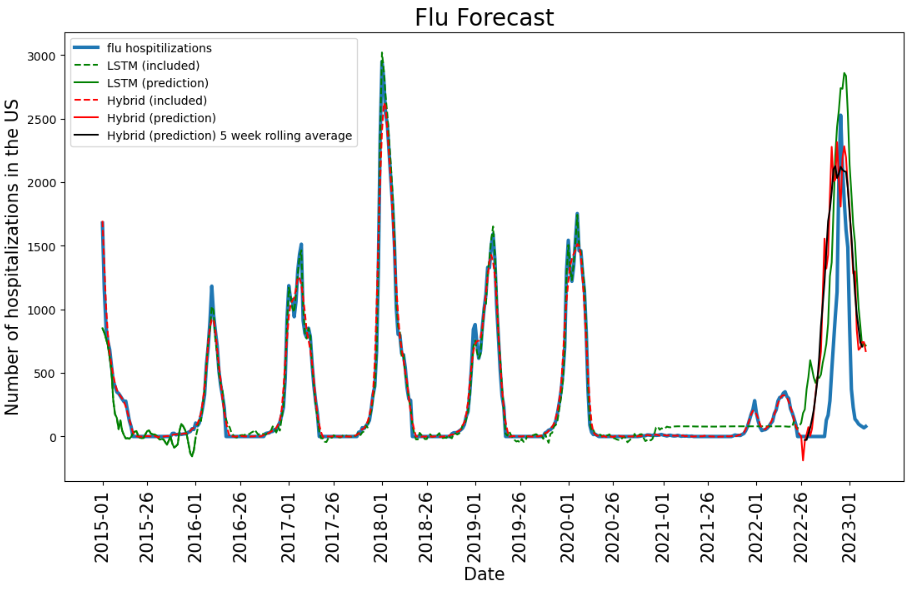
\includegraphics[scale=0.75]{Pictures/flu_models.png}
		\caption{Both models are displayed together, LSTM (green), Hybrid (red), with dashed lines indicated that data was used in training, and solid line represents a prediction.}
		\label{fig:flu_models}
	\end{figure}


\end{document}


